\documentclass[a2paper, 12pt]{article}
\usepackage[font={huge, bf}]{caption}
\usepackage{fontspec}
\setmainfont{Arial}
\usepackage{subcaption}
\usepackage{graphicx}
\usepackage{tikz}
\usepackage{tikzsymbols}
\usetikzlibrary{calc,patterns,shapes.geometric}
\usepackage{float}
\usepackage{pdflscape}
\usepackage{geometry}
\geometry{landscape, margin=2cm}
\captionsetup[subfigure]{justification=justified,singlelinecheck=false}
\pagestyle{empty}

\def\centerarc[#1](#2)(#3:#4:#5){\draw[#1] ($(#2)+({#5*cos(#3)},{#5*sin(#3)})$) arc (#3:#4:#5);}

\begin{document}
	\vspace*{\fill}
	\begin{figure}[!htbp]
		\centering
		\begin{subfigure}[b]{0.48\textwidth}
			\caption{Figure 1}
			\centering
			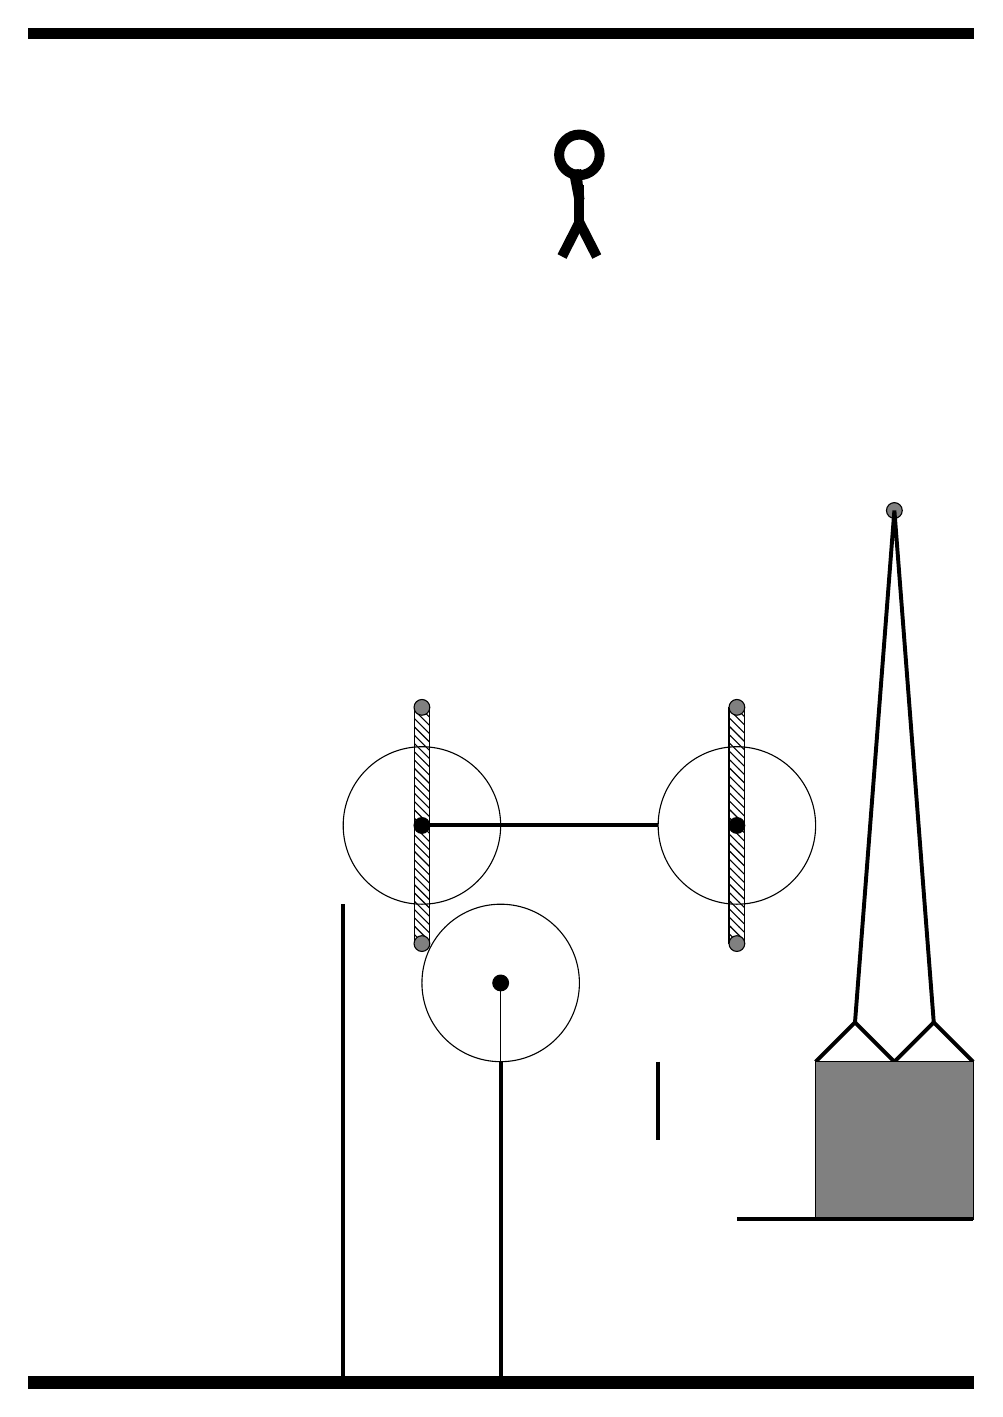
\begin{tikzpicture}
				\draw[fill=black] (-2, 14) rectangle (10, 14.125);
				
				\draw (3,4) circle (1);
				\draw[fill=black] (3,4) circle (0.1);
				\draw[pattern=north west lines, pattern color=black] (2.9,5.5) rectangle (3.1,2.5);
				\draw[fill=black!50] (3,5.5) circle (0.1);
				\draw[fill=black!50] (3,2.5) circle (0.1);
				
				\draw (4,2) circle (1);
				\draw[fill=black] (4,2) circle (0.1);
				\draw (4,-3.15) -- (4,2);
				
				\draw (7,4) circle (1);
				\draw[fill=black] (7,4) circle (0.1);
				\draw[pattern=north west lines, pattern color=black] (6.9,5.5) rectangle (7.1,2.5);
				\draw[fill=black!50] (7,5.5) circle (0.1);
				\draw[fill=black!50] (7,2.5) circle (0.1);
				
				\draw[fill=black!50] (9,8) circle (0.1);
				\draw[line width=0.5mm](8.5,1.5) -- (9,8) --  (9.5,1.5);
				\draw[line width=0.5mm](8,1) --  (8.5,1.5) -- (9,1) -- (9.5,1.5) -- (10,1);
				\draw[fill=black!50] (8, 1) rectangle (10, -1);
				
				\draw[line width = 0.5mm] (3,4) -- (6,4);
				\centerarc[line width = 0.5mm](3,3)(90:180:1);
				\draw[line width = 0.5mm] (2,3) -- (2,-3);
				\centerarc[line width = 0.5mm](3,-3)(180:360:1);
				\draw[line width = 0.5mm] (4,-3) -- (4,1);
				\centerarc[line width = 0.5mm](5,1)(0:180:1);
				\draw[line width = 0.5mm] (6,1) -- (6,0);
				\centerarc[line width = 0.5mm](7,0)(180:270:1);
				\draw[line width = 0.5mm] (7,-1) -- (10,-1);
				
				\node at (5, 12) {\scriptsize \Strichmaxerl[10][-79][96]};
				
				\draw[fill=black] (-2, -3) rectangle (10, -3.15);
			\end{tikzpicture}
		\end{subfigure}
		\hfill
		\begin{subfigure}[b]{0.48\textwidth}
			\caption{Figure 2}
			\centering
			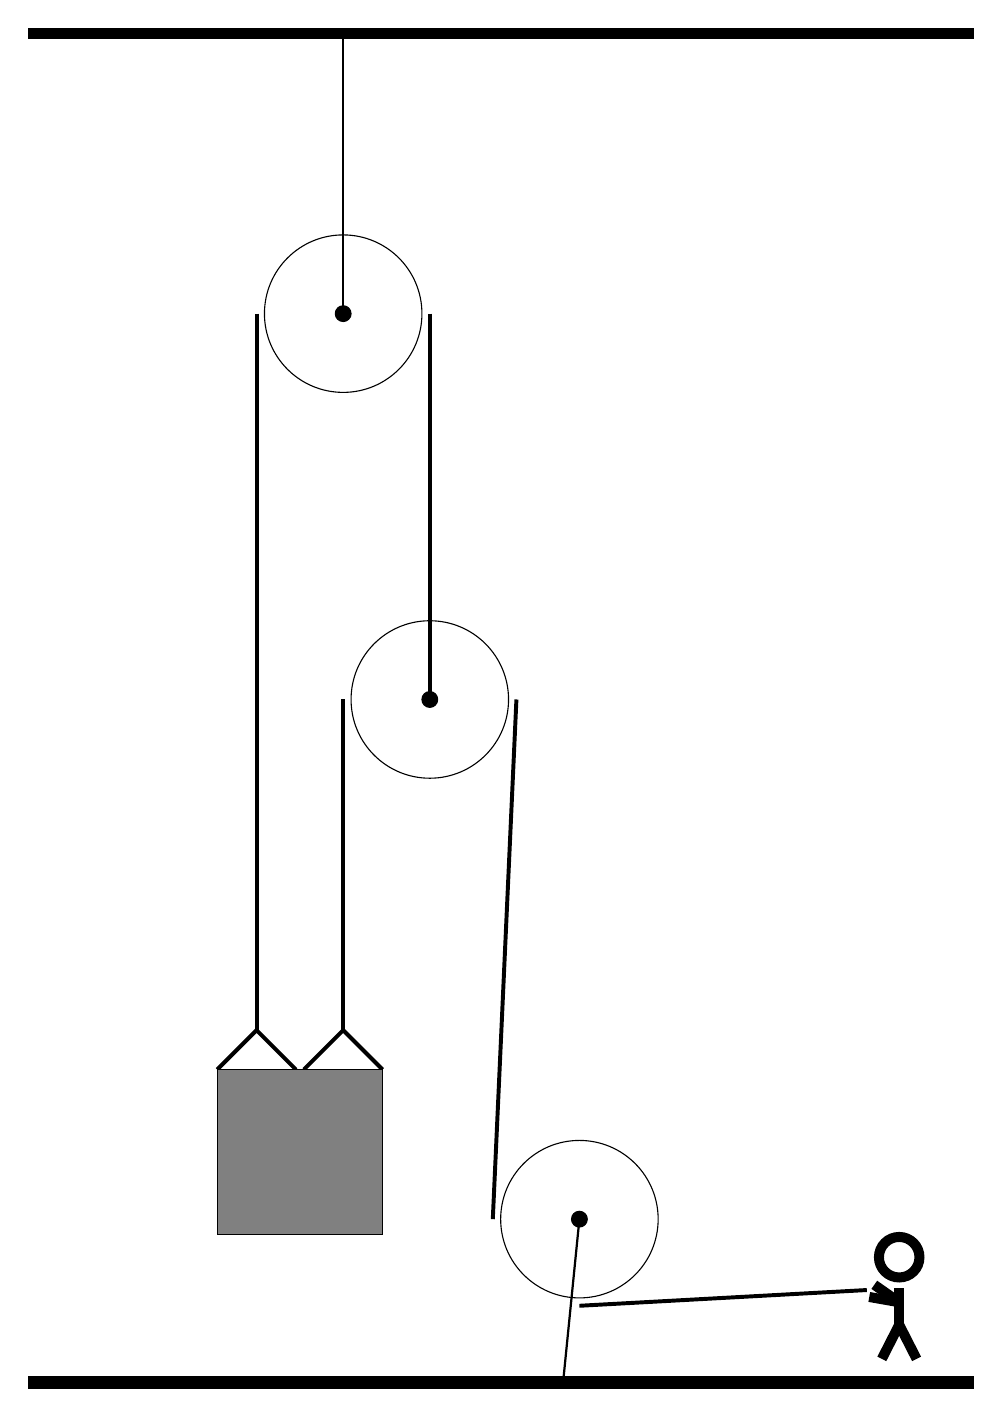
\begin{tikzpicture}
				\draw[fill=black] (-2, 14) rectangle (10, 14.125);
				
				\draw (2, 10.5) circle (1);
				\draw[fill=black] (2, 10.5) circle (0.1);
				\draw[thick] (2, 10.5) -- (2, 14);
				
				\draw (3.1, 5.6) circle (1);
				\draw[fill=black] (3.1, 5.6) circle (0.1);
				
				\draw (5, -1) circle (1);
				\draw[fill=black] (5, -1) circle (0.1);
				\draw[thick] (5, -1) -- (4.8, -3);
				
				\draw[line width = 0.5mm]  (0.4, 0.9) -- (0.9, 1.4) -- (1.4, 0.9);
				\draw[line width = 0.5mm]  (1.5, 0.9) -- (2.0, 1.4) -- (2.5, 0.9);
				\draw[fill=black!50] (0.4, 0.9) rectangle (2.5, -1.2);
				
				\draw[line width = 0.5mm] (0.9, 10.5) -- (0.9, 1.4);
				\centerarc[line width = 0.5mm](2, 10.5)(0:180:1.1);
				\draw[line width = 0.5mm] (3.1, 10.5) -- (3.1, 5.6);
				\draw[line width = 0.5mm] (2.0, 5.6) -- (2.0, 1.4);
				\centerarc[line width = 0.5mm](3.1, 5.6)(0:180:1.1);
				\draw[line width = 0.5mm] (4.2, 5.6) -- (3.9, -1);
				\centerarc[line width = 0.5mm](5, -1)(180:270:1.1);
				\draw[line width = 0.5mm] (5, -2.1) -- (8.65, -1.9);
				
				\node at (9, -2) {\scriptsize \Strichmaxerl[10][-35][170]};
				
				\draw[fill=black] (-2, -3) rectangle (10, -3.15);
			\end{tikzpicture}
		\end{subfigure}
	\end{figure}
		\vspace*{\fill}
\end{document}